\documentclass[12pt, twoside]{article}
\usepackage[letterpaper, margin=1in, headsep=0.5in]{geometry}
\usepackage[english]{babel}
\usepackage[utf8]{inputenc}
\usepackage{amsmath}
\usepackage{amsfonts}
\usepackage{amssymb}
\usepackage{tikz}
\usepackage{yhmath}
\usetikzlibrary{quotes, angles}
\usepackage{graphicx}
\usepackage{enumitem}
\usepackage{multicol}

\newif\ifmeta
\metatrue %print standards and topics tags

\title{Regents Geometry}
\author{Chris Huson}
\date{March 2022}

\usepackage{fancyhdr}
\pagestyle{fancy}
\fancyhf{}
\renewcommand{\headrulewidth}{0pt} % disable the underline of the header
\raggedbottom

\fancyhead[LE]{\thepage}
\fancyhead[RO]{\thepage \\ Name: \hspace{4cm} \,\\}
\fancyhead[LO]{BECA / Dr. Huson / Geometry\\* Unit 9: Algebra\\* 28 March 2022}

\begin{document}
\subsubsection*{9.6 Distance formula, perpendicular and parallel slopes}
\begin{enumerate}
\item Do Now: Graph and label the line segment $\overline{AB}$, $A(1,3)$ and $B(5,9)$.
  \begin{multicols}{2}
    \begin{enumerate}
    \item Mark the midpoint $M$ of $\overline{AB}$. Label it as an ordered pair.  \vspace{1cm} 
    \item Find the slope of $\overline{AB}$
  \end{enumerate} \vspace{1cm}  
  \begin{center} %4 quadrant regents grid
    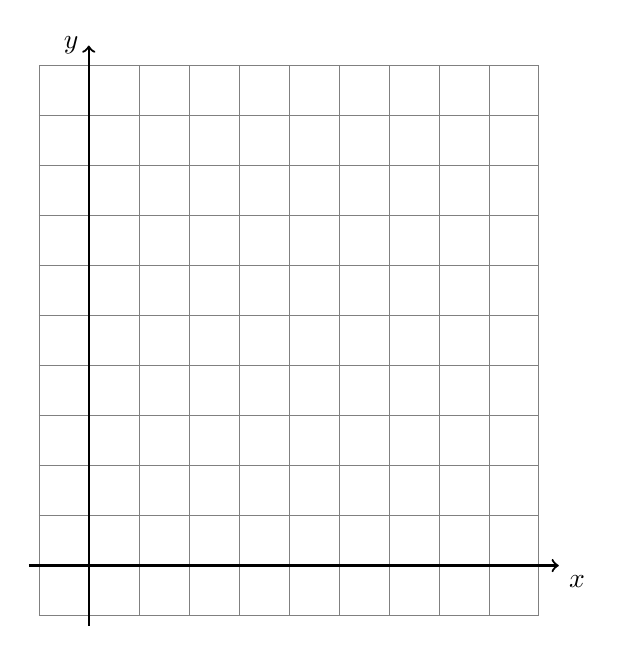
\begin{tikzpicture}[scale=.635]
      \draw [help lines] (-1,-1) grid (9,10);
      \draw [thick, ->] (-1.2,0) -- (9.4,0) node [below right] {$x$};
      \draw [thick, ->] (0,-1.2)--(0,10.4) node [left] {$y$};
    \end{tikzpicture}
    \end{center} 
  \end{multicols}

\item Write down the slope perpendicular to the given slope.
\begin{enumerate}
  \begin{multicols}{2}
    \item   $m= \frac{1}{2} \hspace{1cm} m_{\perp} = $ \vspace{1cm}
    \item   $m= -\frac{3}{5} \hspace{1cm} m_{\perp} = $ 
  \item   $m= -2 \hspace{1cm} m_{\perp} = $ \vspace{1cm}
  \item   $m= 0.75 \hspace{1cm} m_{\perp} = $
  
  \end{multicols}
\end{enumerate} \vspace{1cm}

\item The line $l$ has the equation $y=-\frac{1}{2} x+3$.
\begin{enumerate}
  \item What is the slope of the line $k$, given $k \parallel l$?
  \vspace{1.3cm}
  \item What is the slope of the line $j$, given $j \perp l$?
  \vspace{1.3cm}
\end{enumerate}

%\item What is the slope of a line perpendicular to the line $y=\frac{3}{2}x+1$?  \vspace{1.5cm}
\item Find the slope $m$ of the line $x-2y=1$. Write down $m_{\perp}$.  \vspace{2cm}

\newpage
\item Plot and label the line segment $\overline{PQ}$, $P(-1,8)$ and $Q(7,2)$.
  \begin{enumerate}
    \item Graph the perpendicular bisector of $\overline{PQ}$ and label it with its equation in the form $y=mx+b$.  \vspace{1cm} 
    \item Plot and label $R(6,9)$. Compare the distances $PR$ and $PQ$.
  \end{enumerate} 
  \begin{flushright} %4 quadrant regents grid
  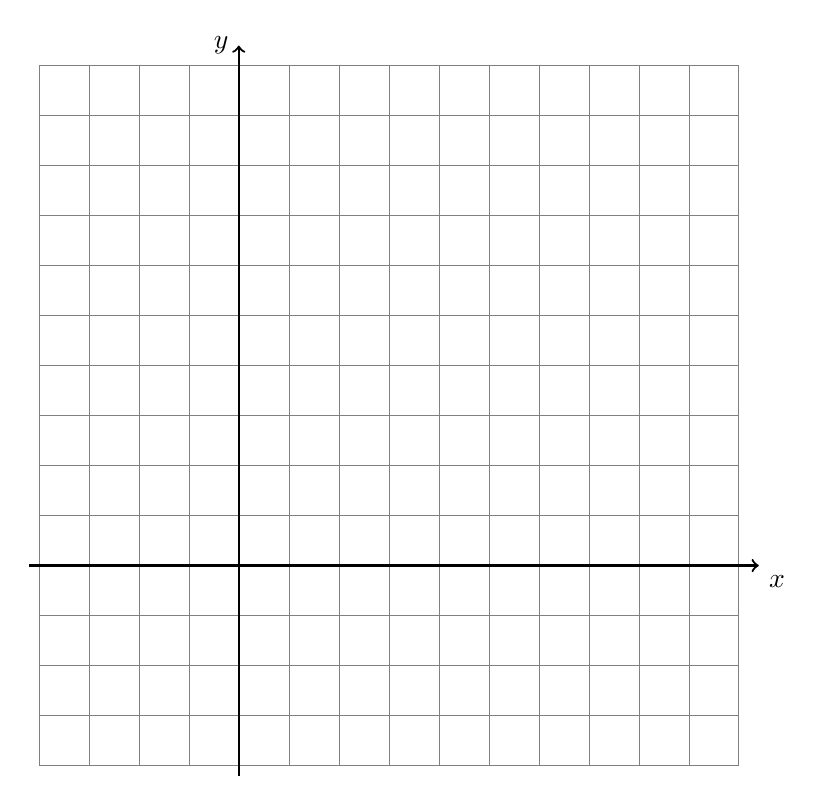
\begin{tikzpicture}[scale=.635]
    \draw [help lines] (-4,-4) grid (10,10);
    \draw [thick, ->] (-4.2,0) -- (10.4,0) node [below right] {$x$};
    \draw [thick, ->] (0,-4.2)--(0,10.4) node [left] {$y$};
  \end{tikzpicture}
  \end{flushright}

\item Solve each system of equations. Check your answer.
  \begin{multicols}{2}
    \begin{enumerate}
      \item \, $4x+8y=20$\\
      $-4x+2y=-30$
      \item \quad $8x+y=-16$\\
      $-3x+y=-5$
    \end{enumerate}
  \end{multicols}
  
\end{enumerate}
\end{document}

\item Find $c$. \\
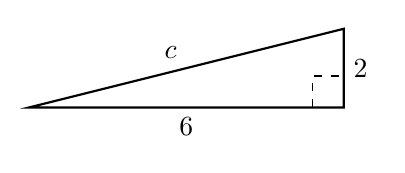
\begin{tikzpicture}[scale=1]
  \node at (2,0.5)[above left]{$c$};
  \node at (4,0.5)[right]{2};
  \node at (2,0)[below]{6};
  \draw [thick] (0, 0)--(4, 0)--(4, 1)--cycle;
  \draw [dashed] (4,0)++(-0.4,0)-- ++(0,0.4)-- +(0.4,0);
\end{tikzpicture} \vspace{1.5cm}

\item What is the length of $\overline{CD}$ if $C(3,1)$ and $D(7,-2)$?\\[0.5cm]
Use $\displaystyle d=\sqrt{(x_2-x_1)^2+(y_2-y_1)^2}$